\documentclass[11pt,a4paper]{report}

\usepackage[titletoc]{appendix}
\usepackage{color}
\usepackage{float}
\usepackage{graphicx}
\usepackage[intoc]{nomencl}
\usepackage{setspace}
\usepackage{pdfpages}
\usepackage{tocbibind}

\newcommand{\quot}[1]{``#1''}
\graphicspath{ {./images/} }

\singlespacing
\boldmath
\setcounter{tocdepth}{4}
\makenomenclature


\begin{document}
	
\includepdf{cover}
	
	
	\begin{abstract}
		This is the abstract.
	\end{abstract}
	
	
	\tableofcontents

	\printnomenclature
	\listoffigures
	\listoftables
	
	
	\chapter{Introduction}
		\nomenclature{y}{A very cool variable.}
		\section{Background}
		Artificial neural networks in all their various incarnations have been successfully used to solve a very wide range of machine learning problems, thanks to their good representational capabilities \cite{sharma2010constructive}.
		
		Theoretically, a simple feed-forward neural network with a single hidden layer and a sufficient number of neurons in that layer is an universal approximator \cite{hornik1989multilayer,kuurkova1992kolmogorov}. In practice however, too small networks may be unable to adequately learn the problem, while overly large networks tend to overfit the training data \cite{parekh2000constructive}.
		
		The problem of determining the optimal neural network topology is thus very important. However, there are currently no efficient methods to choose \emph{a priori} the best network architecture for a given problem \cite{parekh2000constructive}. In real-world applications, \emph{trial-and-error} and decisions based on previous knowledge about the problem are often the preferred approach. The chosen architecture has thus no guarantees to be the optimal one for the task \cite{sharma2010constructive}.
		
		To overcome this problem, solutions that involve learning both the\\weights of the synapses \emph{and} the network topology have been suggested \cite{parekh2000constructive}.
		
		One of the proposed answers is the class of algorithms of the so-called \emph{constructive neural networks}. The main idea behind it is starting from a minimal architecture and then adding hidden layers, nodes and connections during training \cite{kotsiantis2007supervised,sharma2010constructive}.
		
		Such algorithms provides the flexibility to explore the space of neural network topologies in a controlled, \emph{data-driven} fashion. Furthermore, because small solutions are found first, this method has the potential to discover near-minimal networks that approximately match the complexity of the learning task \cite{parekh2000constructive}.
		
		For all these reasons, applying a constructive approach to existing learning algorithms constitutes an interesting problem.
		
		\newpage
		
		In the present project I worked on the development of a constructive version of the DIM\footnote{Divisive Input Modulation.} learning algorithm, as described in \cite{spratling2009unsupervised}, and its derivation \cite{spratling2012unsupervised} used in the \emph{non-linear} PC/BC model\footnote{Predictive Coding as Biased Competition} \cite{spratling2008predictive}. The original algorithm has been developed to train a variation of \emph{negative feedback networks} and has proven to be very successful in the unsupervised learning of image components, yielding state-of-the-art performances in various benchmarks, even in the presence of occlusion and overlapping \cite{spratling2009unsupervised}.
		
		On one hand, the main feature of negative feedback networks is the competition between nodes, which enables them to be selective for different input stimuli by making the individual synaptic weights more distinct. This is achieved by having inhibiting (\emph{divisive}) feedback connections from the output neurons back to their input nodes \cite{spratling2009unsupervised}. 
		
		On the other hand, the PC model proposes a hierarchical architecture in which alternating populations of \emph{error-detecting} and \emph{predicting} nodes interact with each other to carry out the perception process \cite{spratling2014predictive}. In particular, the higher levels of the network are not limited to passively receiving the input from the preceding nodes, but instead they actively predict the input they expect to receive. Feedback connections convey the predictions, while feedforward connection transmit the residual error between those predictions and actual input \cite{spratling2008predictive}.

		\begin{itemize}
			\item Show some images of the network structure.
			\item Make clear that x to e is one-to-one while e to y is many-to-many.
			\item Talk about the dictionary approach? (very briefly?)
		\end{itemize}

		A connection can be drawn between these two models. If we consider negative feedback networks from an equivalent perspective, namely a generative one, it can be shown that the higher level of the network produces a \emph{reconstruction} of the input via the feedback connections; while feedforward connections instead convey \emph{residual error} between the top-down prediction and the bottom-up input \cite{spratling2009unsupervised}, much like in the PC model.
		Symmetrically, \emph{Predictive Coding} can be redefined as a form of \emph{Biased Competition} \cite{spratling2008predictive}.
		
		Algorithms that work for one model can thus be adapted to work for the other one. In particular, PC/BC networks trained using the DIM algorithm are referred to as PC/BC--DIM. Most notably, in this model the training of the weights of feedforward and feedback connections can be performed simultaneously and independently, thus providing a biologically sound computational theory explaining how reciprocal connections are learnt in actual cortical areas \cite{callaway1998local,spratling2012unsupervised}.
		
		\section{The project}
		The main focus of the project has been in improving the PC/BC--DIM algorithm with the ability to progressively grow a near-optimal network topology alongside the feedforward and feedback weights. In the process, I also implemented a constructive version of the basic DIM algorithm.
		
		The project aim is to provide an enhanced version of the original algorithm which performs equally well but produces smaller networks that can be trained faster.
		
		The structure of the problem is well suited for the design of a constructive variant. The network is fully connected between the error-detecting and the prediction layers, so there is no need to consider all the possible partial connections \cite{?}.
		
		In the context of image decomposition, the pixel values act as the input which is fed to the error-detecting neurons, while the output of the nodes in the predictive layer represents the degree by which that component participates to the generation of the image. According to this interpretation, the weights associated to the connections targeting each prediction neuron are thus a \quot{basic vector}, or \quot{elementary component} of the images to be reconstructed \cite{spratling2014predictive}.

		Furthermore, the number of neurons in the error layer is fixed to the number of input units. Thus the algorithm regulating the evolution of the network has to focus only on the output layer, by tuning its number of neurons when deemed necessary. That corresponds to determining the number of distinct components which are needed to decompose the images in the training set. As already stated, this value is in general not known \emph{a priori}, and it has been the obvious target of the implemented algorithm.
		
		Any type of constructive algorithm needs some kind of way to measure the error of the network to be able to decide whether and when adding a neuron to it. Conveniently, in the present case that quantity is embedded directly into the network itself, in the form of its error-detection layer. I performed experiments with different sets of criteria based on this measure, starting with those available in the literature describing the state-of-the-art, and modifying them and fine-tuning them to better fit the problem at hand.
		
		Tested with some standard benchmarks, specifically the \emph{bars} \cite{spratling2012unsupervised} and \emph{squares} problem \cite{spratling2009unsupervised}, the developed constructive algorithm has reported state-of-the-art results on the same level of accuracy of the original, while at the same time consistently building smaller networks.
		
		In summary, the work conducted for this project represents a sensible improvement over the
		state-of-the-art DIM algorithm in term of training times and optimality of the size of the network.

		\section{Structure of the report}
		The main part of the report is structured as follows:
		\begin{itemize}
			\item Chapter 1 acts as an introduction to the project, its goals and the problem it solves;
			\item Chapter 2 provides a survey of the literature, with references to the relevant choices made during the project's undertaking;
			\item Chapter 3 describes the work conducted in full detail and evaluates the results against the other algorithms described in the literature review;
			\item Chapter 4 concludes the body of the document by summarizing the main points of the work and pointing at possible future developments.
		\end{itemize}
		A list of the bibliographic references and an appendix containing the whole source code of the project terminate the report.
	
	
	\chapter{Literature Review}
		\section{Artificial Neural Networks}
		\emph{Artificial neural networks} are a model designed to mimic the way in which the brain performs a task, usually simulated in software on a computer. Neural networks are parallel machines built upon simple, massively interconnected computing cells called \emph{neurons} (figure~\ref{fig:multilayer}). Every connection between nodes (\emph{synapse}) has an associated \emph{weight} \cite{haykin2009neural}.
		
		\begin{figure}[h]
			\centering
			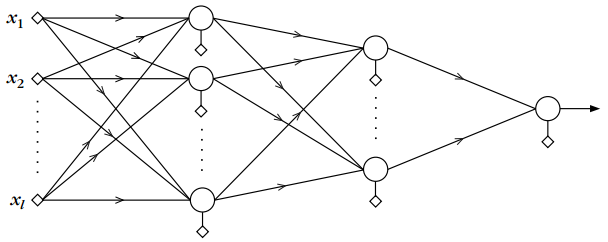
\includegraphics[width=\textwidth]{multilayer}
			\caption{Architecture of an artificial neural network with two hidden layers and a single output neuron \cite{theodoridis2008pattern}.}
			\label{fig:multilayer}
		\end{figure}		
		
		The way in which neural networks are usually programmed to perform a function is through a process of \emph{learning}, which typically involves modifying the synaptic weights in such a way as to attain the desired objective \cite{haykin2009neural}. As will be analysed in section~\ref{sec:constructive}, learning is not limited to that, as it is also possible for neural networks to modify their own topology, ability which is exploited by the current project.
		
		\newpage
		
		\begin{figure}[t]
			\centering
			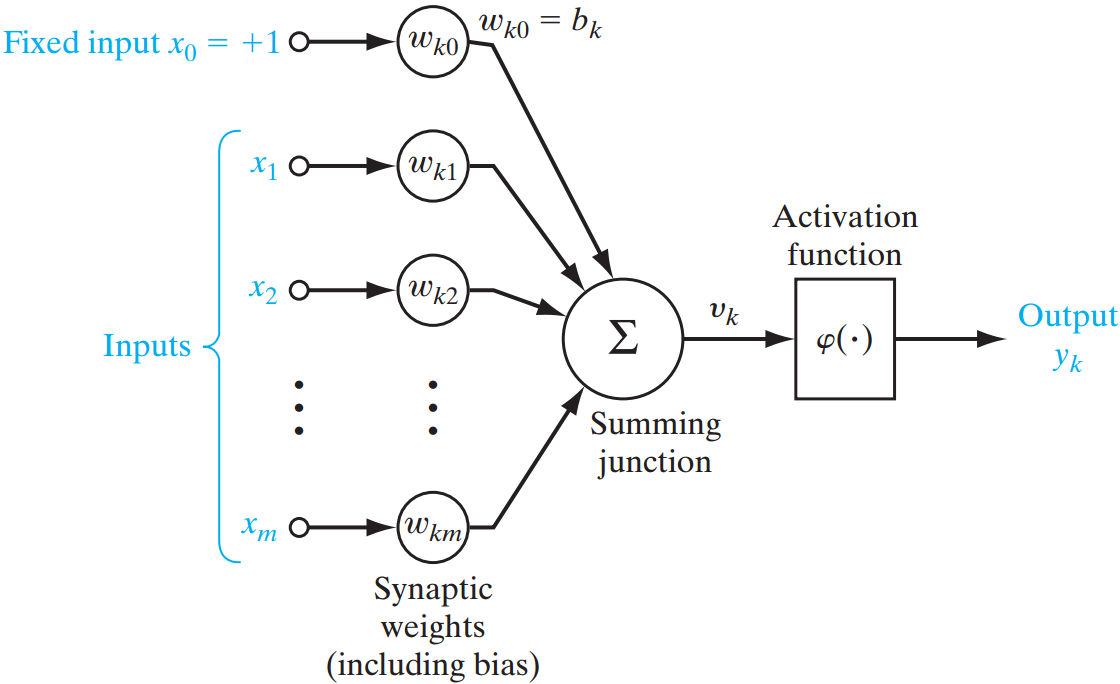
\includegraphics[width=0.85\textwidth]{neuron}
			\caption{Nonlinear model of a neuron \cite{haykin2009neural}.}
			\label{fig:neuron}
		\end{figure}
		
		Figure~\ref{fig:neuron} shows a representation of a generic model of an artificial neuron. In detail, its main components are:
		\begin{enumerate}
			\item A set of \emph{synapses} or \emph{connecting links}, characterized by a \emph{weight} or \emph{strength}. If a signal $x_j£$ is at the input of a synapse $j$ connected to a neuron $k$, the input signal gets multiplied by the synaptic weight $w_{kj}$.
			\item A \emph{sum} function $\Sigma$ which implements a \emph{linear combination} of the inputs with their respective synaptic weights.
			\item An \emph{activation} or \emph{transfer} function $\varphi$ which limits the amplitude of the output of the neuron, usually to the closed interval $[-1, 1]$. Nonlinear functions such as the \emph{sigmoid} are common choices.
			\item Optionally, the model can include a value $b_k$ called \emph{bias}, whose role is to increase or lower the net input of the activation function. This is usually implemented by having an additional, fixed input $x_0 = 1$ multiplied by its respective weight $w_{k0}$ \cite{haykin2009neural}.
		\end{enumerate}
		
		Mathematically, the behaviour of a neuron can be described by the following equations:
		\begin{equation}
			v_k = \sum_{j=0}^{m} w_{kj}x_j
		\end{equation}
		\begin{equation}
			y_k = \varphi(v_k)
		\end{equation}
		
		Nodes in a network are usually grouped into three classes: an \emph{input layer}, whose neurons receive the information to be processed; an \emph{output layer}, which yield the results of the processing; and neurons in between organized in zero or more \emph{hidden layers} \cite{kotsiantis2007supervised}.
		
		The representational power of neural networks is well defined theoretically: in fact, any continuous function can be implemented in a three-layer net, given sufficient number of hidden units, proper nonlinearities, and weights \cite{hornik1989multilayer,kuurkova1992kolmogorov,lam2015prslides}.
		
			\subsection{Network architectures}
				\subsubsection{Feedforward networks}
				The simplest type of topology is the feedforward network, which allows signals to travel only one way, from input to output \cite{kotsiantis2007supervised}; this layout is thus strictly acyclic. The signals resulting from the input layer are fed to the second layer, and so on till the final layer, whose output constitutes the overall response of the network to the source pattern \cite{haykin2009neural}.
				
				\begin{figure}[h]
					\centering
					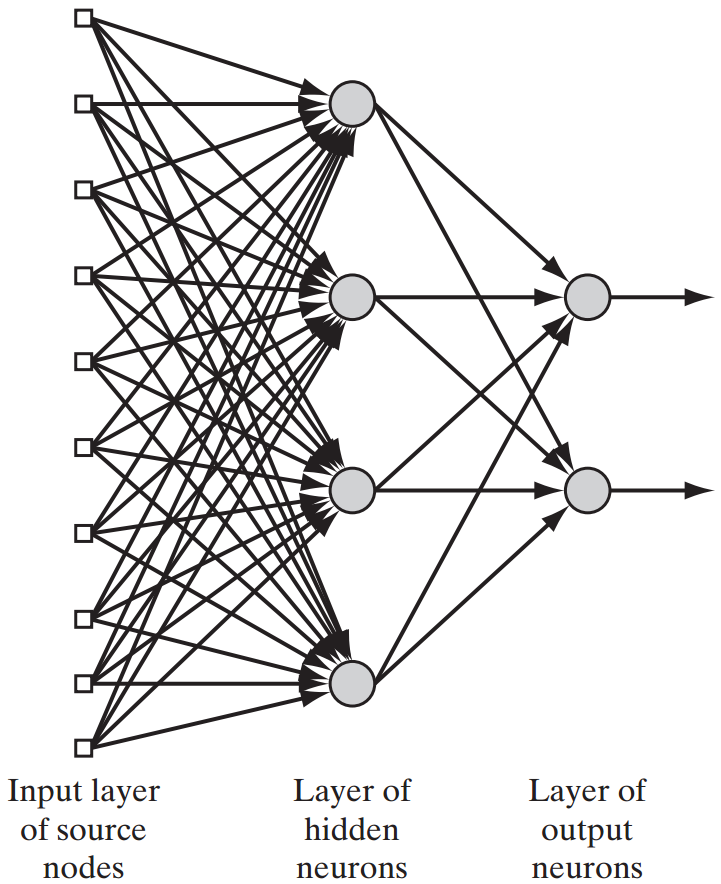
\includegraphics[width=0.6\textwidth]{feedforward}
					\caption{Fully connected feedforward neural network \cite{haykin2009neural}.}
					\label{fig:feedforward}
				\end{figure}
				
				Typically (but not necessarily) the neurons in each layer are only connected to the ones into the immediately following layer. If every node in each layer is connected to every other node in the adjacent layer, the neural network is said to be \emph{fully connected} (respectively \emph{partially connected}) \cite{haykin2009neural}. Figure~\ref{fig:feedforward} shows an example of such a network.
				
				\subsubsection{Recurrent networks}
				\begin{figure}[t]
					\centering
					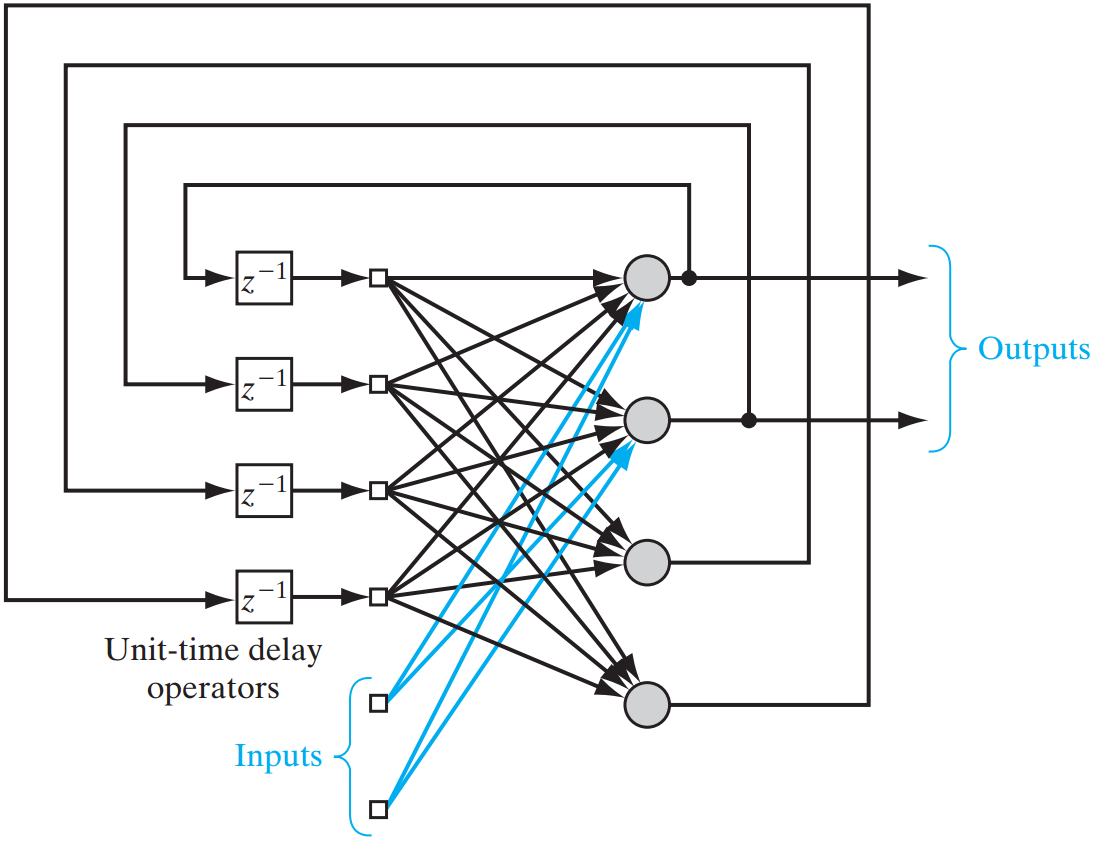
\includegraphics[width=0.9\textwidth]{recurrent}
					\caption{Recurrent neural network with hidden neurons \cite{haykin2009neural}.}
					\label{fig:recurrent}
				\end{figure}
				Contrarily to feedforward networks, \emph{recurrent} neural networks have at least one \emph{feedback} loop. Feedback is present in a system when the output of an element influences (at least in part), the input applied to that same element. The presence of feedback loops has a deep impact on the learning capabilities of a network \cite{haykin2009neural}. Specifically, recurrent neural networks gain the ability to predict element in sequences on the basis of their predecessors. \cite
				
				\subsubsection{Deep or hierarchical networks}
		
			\subsection{Training algorithms}
				\subsubsection{Supervised learning}
				\subsubsection{Unsupervised learning}
		
		\section{Negative Feedback Networks}
		The main idea.
			\subsection{Fyfe's Network}
			\subsection{Harpur's Network}
	
		\section{Non-negative Matrix Factorisation}
		Image decomposition, main algorithm
			\subsection{Sequential version}
	
		\section{Divisive Input Modulation}
		This.

		\section{PC/BC}
			\subsection{Predictive coding}
			\subsection{Predictive coding as biased competition}
			\subsection{PC/BC--DIM}
			
		\section{Constructive Neural Networks}
		\label{sec:constructive}

	
	\chapter{Main Result}
		\section{Theoretical Development}
		\section{Analysis and Design}
		\section{Implementation and Experimental Work}
		\section{Results}
		\section{Discussion}
		
	\chapter{Conclusion}
	
	\bibliographystyle{plain}
	\bibliography{references}
	\nocite{*}
	
	\begin{appendices}
		\chapter{Source Code}
	\end{appendices}
\end{document}
